\chapter{Diskussion}\label{chap:Diskussion}
\section{Aussagekraft des SIR-Modells}
In \autoref{fig:SIR_Deutschland} sind die drei Kennzahlen für das SIR-Modell dargestellt. Die R-Wert Berechnung des Robert-Koch-Instituts basiert auf den selben Daten \autocite{}, jedoch werden hierfür noch einige weitere Maßnahmen und Annahmen getroffen, welche das Maß dieser Bachelorarbeit sprengen würden.
Wie auch in den Veröffentlichungen und \autoref{sec:Resultate-SIR} beschrieben, weisen die Meldungen der Daten überraschend viele Fehler auf: 

Und dies sind lediglich die automatisch festgestellten Fehler. Inwiefern die Daten nicht das Infektionsverhalten wiederspiegeln, lässt sich anhand der wöchentlichen Schwankungen der Infizierendenzahl abschätzen: Vermutlich werden am Wochenende weniger Tests durchgeführt oder weniger Meldungen abgegeben. 
Zudem spiegeln die Zahlen nur die getesteten Fälle wieder. Somit kann zum einen verstärktes Testen zu späteren Zeiträumen in der Pandemie die Zahlen verfälschen und zum anderen machen symptomfreie Krankheitsverläufe es schwer, festzustellen ob und wie lange eine Person infektiös war.

Da die Anzahl der Infizierenden in einem SIR-Modell sehr klein ist und daher kleine Unregelmäßigkeiten eine große Auswirkung haben, lässt sich anhand dieses simplen SIR-Modells keine stichfeste Aussage treffen.
Im Rahmen dieser Arbeit dient es als Mahnmal, dass die erwähnten Probleme stets beachtet werden müssen:
Die täglichen Schwankungen werden dadurch ausgeglichen, dass die 7-Tages Inzidenz verwendet wird. Die Verwendung von den täglichen Fallzahlen des RKIs als offizielle Stelle sorgt für eine Vorsortierung der Meldungen. Zudem werden im weiteren Verlauf ausschließlich die Fallzahlen benutzt, da diese höchste Größenordnungen erreichen und daher Inkonsistenzen von einigen 100 Fällen pro Tag weniger verheerend sind.
\todo{Vergleiche mit (kommentar siehe Code) Quelle einpflegen}
\todo{Eventuell anregung aus dem Video zu SIR einbinden}
% https://www.rki.de/DE/Content/Infekt/EpidBull/Archiv/2020/Ausgaben/17_20.pdf?__blob=publicationFile

\section{Zusammenhänge von Bevölkerungsdichten und Corona-Zahlen der Landkreisen}\label{sec:discussion:pop_density}
Klar zu erkennen in \autoref{fig:distribution_pop_density_counties} sind die vielen kleinen roten Punkte, welche die Stadtkreise kennzeichnen, wie auch im Anhang in \autoref{tab:counties_by_pop_density} klar zu erkennen.
Diese sind jedoch oftmals von Landkreisen mit vergleichbar niedrigen Bevölkerungsdichten (außer im Rhein-Ruhrgebiet) umgeben. Daher lässt sich systematisch nur sehr schwer zwischen Landkreisen mit wirklich niedriger Bevölkerungsdichte unterscheiden und Landkreisen mit niedriger Bevölkerungsdichte, welche eine Stadt umschließen und eine deutlich höhere Bevölkerungsdichte aufweisen würden, wenn die Stadt zum Landkreis gehören würde. Da somit manche mittelmäßig dicht bevölkerte Gebiete nicht trivial in einen stark bevölkerten Stadtkreis und einen dünn bevölkerten Landkreis zerlegt sind, lassen sich keine Schlussfolgerungen ziehen, inwiefern dünn bevölkerte Gebiete stärker betroffen sind als dichter bevölkerte Gebiete, dies spiegelt sich auch in den im Vergleich zu den restlichen Matrizen recht homogenen Matrizen in \autoref{fig:matrizes_pop_density_counties} wieder.
Jedoch lässt sich die Aufteilung vorzüglich nutzen, um festzustellen, ob die 7-Tages Inzidenzen einer Stadt vor den 7-Tages Inzidenzen im Umland steigen.
\autoref{fig:highest_selected_counties} zeigt jedoch eindeutig, das die 7-Tages Inzidenzen der gewählten Städte und Landkreise außergewöhnlich zeitgleich steigen und fallen: Die höchste Korrelationswahrscheinlichkeit bei einer Verschiebung von $\tau=0$ bei 50\% ist derart über dem nationalen Durchschnitt von ca. 8,7\%, das davon ausgegangen werden kann, das sich ein Landkreis, der eine Stadt komplett umgibt einen sehr ähnlichen Verlauf der 7-Tages Inzidenz aufweisen wird.
Auch die sehr kleinen in \autoref{fig:sum_selected_c} eingetragenen Differenzen zwischen dem Durchschnitt der Korrelationswahrscheinlichkeiten der positiven Verschiebungen und dem Durchschnitt der Korrelationswahrscheinlichkeiten der negativen Verschiebungen: die maximalsten Differenzen entsprichen lediglich 10\% des Maximalwerts und sind ausgeglichen oberhalb und unterhalb der null angeordnet.

Da die Inzidenzwerte jedoch zuvor normiert wurden und wie in \autoref{fig:germany_incidence} zu sehen manche Städte deutlich stärker als ihr Umland betroffen waren - oder umgekehrt - lässt sich dies nicht über die absoluten Werte sagen, sondern lediglich über die Anstiege und Abnahmen sagen.
Zudem ist die geringe Größe der Teilmenge mit 18 untersuchten Paaren stets zu berücksichtigen, auch wenn kein trivialer Zusammenhang zwischen dem Ergebnis und der Auswahlmethode besteht. Es wurden die Städte gewählt. welche vollständig von einem Landkreis umgeben sind,

\section{Zusammenhänge von Bevölkerungsdichten und Corona-Zahlen der Regierungsbezirke}
Um das oben beschriebene Problem von nicht trivial aufgeteilten Gebieten zu beheben und einen Zusammenhang zwischen Bevölkerungsdichten und Corona-Zahlen herstellen zu können, werden statt der Landkreise die Regierungsbezirke verwendet.

Alle Matrizen in \autoref{fig:matrizes_pop_density_districts} scheinen einen Farbverlauf von links unten nach rechts oben zu besitzen, in der Matrix rechts oben ist es am deutlichsten ersichtlich. Dies spricht stark dafür, dass die 7-Tages Inzidenz der bevölkerungsdichten Regierungsbezirke früher ansteigt. Der Farbverlauf wirkt relativ kontinuierlich, was den Verdacht auf einen Zusammenhang noch weiter verstärkt.

Dieser Effekt entspricht durchaus der ersten Intuition, da sich, wie der Name schon sagt, in dichter bevölkerten Gebieten mehr Menschen auf engerem Raum bewegen und dadurch von mehr Infizierenden schneller angesteckt werden.
Zudem sind die Treffpunkte in Städten vermutlich deutlich größer: Größere Unternehmen, Universitäten, größere Diskotheken, größere Wohneinheiten, stärker frequentierte Knotenpunkte des Nah- und Fernverkehrs etc. Dadurch kann es zu mehr und stärkeren Superspreading-Events, Ereignisse, an denen sich eine Vielzahl an Menschen an wenigen Infizierten ansteckt, kommen.

Die Superlative dieser Superspreading-Events stören jedoch auch die Regelmäßigkeit des angesprochenen Farbverlaufs in den Matrizen: Beispielsweise kam es laut Zeit \autocite{} im Oktober 2020 im Landkreis Cloppenburg zu einem Corona Ausbruch in einem Schlachthof. Erstellt man für den 06.10.2020 und den 07.10.2020 eine Karte mit allen Landkreisen mit einer 7-Tages Inzidenz über 50 rot ein, ergibt sich die Karte in \autoref{fig:oktober_inzidenzen_uber_50}. 

\todo{Zeit Artikel referenzieren, siehe hier Kommentar:}
% https://www.zeit.de/news/2020-10/09/corona-zahlen-im-kreis-cloppenburg-hochgeschnellt
\begin{figure}
    \centering
    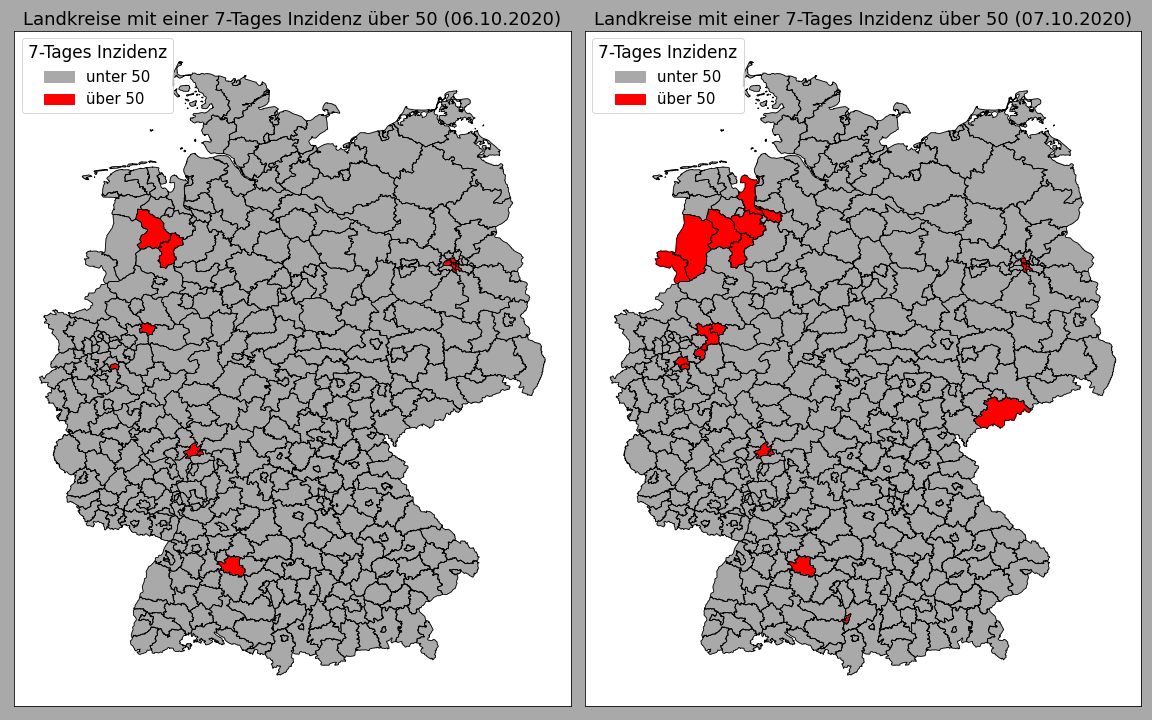
\includegraphics[width=0.95\textwidth]{figures/Diskussion/Inzidenzen_uber_50_oktober_2020.png}
    \caption{Die Deutschlandkarte, rot eingefärbt jeweils die Landkreise mit einer 7-Tages Inzidenz am 06.10.2020 beziehungsweise 07.10.2020 über 50.}
    \label{fig:oktober_inzidenzen_uber_50}
\end{figure}
Klar erkennbar: Die extrem starke Ausbreitung des Corona-Viruses in diesem Gebiet. Vermutlich sorgte der Corona Ausbruch in Cloppenburg für einen rapiden Anstieg in diesem Gebiet in diesem Zeitraum, in welchem die Anomalie in der Matrix begründet liegt. In \autoref{fig:cloppenburg} ist zudem klar ersichtlich, das die 7-Tages Inzidenz in Cloppenburg nur in diesem Zeitraum zu den höchsten zählte und sich anschließend eher im Mittelfeld bewegte.

\begin{figure}
    \centering
    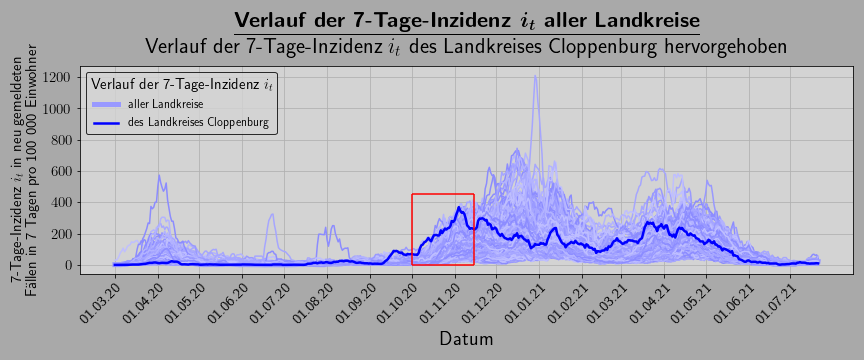
\includegraphics[width=0.95\textwidth]{figures/Diskussion/Inzidenz_Cloppenburg.png}
    \caption{Die 7-Tages Inzidenzen der deutschen Landkreise, in Blau die 7-Tages Inzidenz von Cloppenburg.}
    \label{fig:cloppenburg}
\end{figure}

Jedoch muss nicht immer ein außerordentlicher Corona Ausbruch für eine auffällige Färbung in der Matrix sorgen: Die vierte Zeile in den Matrizen, welche dem Regierungsbezirk Trier zugeordnet ist, ist erstaunlich dunkel.
Vergleicht man den Inzidenzverlauf des Regierungsbezirks mit den Inzidenzverläufen der restlichen Regierungsbezirke, scheint die 7-Tages Inzidenz des Regierungsbezirkes Trier zu Beginn durchschnittlich früh und stark angewachsen zu sein wie die restlichen, was gegen ein markantes Superspreading-Event spricht. Im Vergleich zu den anderen Regierungsbezirke blieb die 7-Tages Inzidenz jedoch ungewöhnlich stabil, wie in Abbildung \autoref{} zu sehen. Die insgesamt niedrige Summe aller täglichen 7-Tages Inzidenzen des Regierungsbezirks, welche in \autoref{fig:distribution_incidences_districts} erkennbar ist, stützt diese These, das die 7-Tages Inzidenz im nationalen Vergleich zwar früh stieg, aber durchgehend bei relativ niedrigen Werten blieb.

\begin{figure}
    \centering
    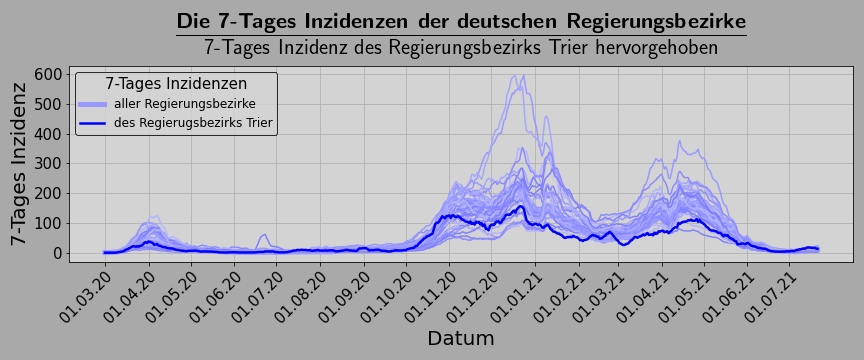
\includegraphics[width=0.95\textwidth]{figures/Diskussion/Inzidenz_Trier.png}
    \caption{Der Verlauf der 7-Tages Inzidenzen der deutschen Regierungsbezirke. Der Verlauf des Regierungsbezirks Trier ist blau hervorgehoben.}
    \label{fig:my_label}
\end{figure}



Die Schlussfolgerungen, welche anhand der Matrizen aufgestellt wurden, werden auch von \autoref{fig:average_shift_districts.png} und \autoref{fig:positive_or_negative_shift_districts} gestützt: Bis auf die beiden erwähnten Ausnahmen, ähneln die beiden Deutschlandkarten \autoref{fig:distribution_pop_density_districts}.

\section{Zusammenhänge von Gemeindeschlüssel und Corona-Zahlen der Landkreise und Regierungsbezirke}
Die Matrizen aus \autoref{fig:matrizes_north_to_south_counties} und \autoref{fig:matrizes_north_to_south_districts} zeigen keinen konstanten Farbverlauf: Viel eher sind die obersten Zeilen bis auf wenige Ausnahmen sehr hell, sie sind den neuen Bundesländern, Schleswig-Holstein und dem Saarland zugeordnet. Der mittlere und untere Teil, welche grob den Gebieten der alten Bundesländer zugeordnet sind, sind eher dunkler.

Der dunkle Strich in der dritten Zeile der Matrizen in \autoref{fig:matrizes_north_to_south_districts} ist Berlin zugeordnet. Die Interpretation dieser Zeile findet sich in \autoref{sec:discussion:pop_density}. Hamburg, welches für den dunklen Strich in den selben Matrizen in Zeile 11 verantwortlich ist, fällt in die selbe Kategorie.

Das Saarland, welches in \autoref{fig:matrizes_north_to_south_districts} laut \autoref{tab:districts_by_admunitid} der zweiten Zeile zugeordnet ist, ist in in allen Matrizen in der oberen Hälfte eine der dunkleren Linien, im unteren Teil würde sie vermutlich nicht auffallen.
Dies ist wenig verwunderlich, da das Saarland bei der Sortierung nach dem Gemeindeschlüssel am auffälligsten aus dem Nord-Süd- und Ost-West-Raster herausfällt, wie in \autoref{fig:distribution_AdmUnitId} zu sehen.

Somit scheinen die 7-Tages Inzidenzen in den alten Bundesländern vor den 7-Tages Inzidenzen in den neuen Bundesländern zu steigen.


\section{Durchschnittliche Verschiebung im nationalen Vergleich Landkreise}
\autoref{fig:average_shift_counties.png} und
\autoref{fig:positive_or_negative_shift_counties} weisen die selben Merkmale auf wie die analysierten Abbildungen  und stützen daher die genannten Thesen.
